\documentclass[11pt]{article}
\usepackage{xcolor}
\usepackage{listings}
\usepackage{graphicx}
\usepackage{url}
\usepackage{multicol}
% Define a custom color for the terminal command
\definecolor{terminalcolor}{RGB}{0, 128, 0}

% Define a custom command for highlighting terminal commands
\newcommand{\terminal}[1]{\texttt{\color{terminalcolor}#1}}

\begin{document}

\begin{titlepage}
    \begin{center}
        
\includegraphics[scale=0.35]{du_logo.png}\par
        \begin{Huge}
            \textsc{University of Dhaka}\par
        \end{Huge}
        \begin{Large}
            Department of Computer Science and Engineering\par \vspace{1cm}
            CSE-3111 : Computer Networking Lab \\[12pt]    
            Lab Report 1 : An Exercise on LAN Configuration and Troubleshooting Tools
        \end{Large}
    \end{center}
    
    \vfill
    
    \begin{large}
        \begin{multicols}{2}
            \noindent
            \textbf{Submitted By :\\[12pt]}
                Name: Md. Emon Khan\\[8pt]
                Roll No : 30\\[12pt]
                Name: Mahmudul Hasan\\[8pt]
                Roll No : 60\\[12pt]
                
            \columnbreak
            
            \noindent
            \textbf{Submitted To :\\[12pt]}
                Dr. Md. Abdur Razzaque\\[12pt]
                Dr. Md. Mamun Or Rashid\\[12pt]
                Dr. Muhammad Ibrahim\\[12pt]
                Md. Redwan Ahmed Rizvee
        \end{multicols}    
    \end{large} 
\textbf{Submitted On :} January 26, 2024\\[20pt]

\end{titlepage}

\section{Introduction}
The primary objective of Lab Experiment-1 is to get a quick introduction to LAN configuration and troubleshooting tools using command line with tools like PING, Traceroute, ARP, Static routing, netstat, ifconfig, nslook, etc.

\subsection{Objectives}
Some of the specific objectives of the lab experiment are:
\begin{itemize}
    \item List a few commands recommended by the teacher and try them out in the cmd
    \item Understand how and what information each of the commands give, or what tasks may be done by them
    \item Note how the given information may be beneficial in the context of computer networking
\end{itemize}

\section{Theory}
 Devices receive local addresses within their LANs, and routers connect local networks to broader networks using public addresses. These processes adhere to specific protocols. Troubleshooting and configuring LANs and connected devices involve using various tools.


\section{Methodology}

During the lab session, we systematically executed each command to explore their functionalities. Some commands offered different options, prompting us to experiment with variations. We tested the addresses of other devices within the LAN and also probed various internet websites. Notably, we extracted and scrutinized diverse network configurations and usage statistics using the employed commands.

\newpage
\section{Experimental result}

Some Snapshots of the terminal output for each of these tools. 

\subsection{Ping}
The \terminal{ping} command is commonly used to test the reachability of a host on an Internet Protocol (IP) network and to measure the round-trip time for messages sent from the originating host to a destination computer.
\subsubsection{Basic Ping: \terminal{ping du.ac.bd}}
\begin{figure}[!h]
    \centering
    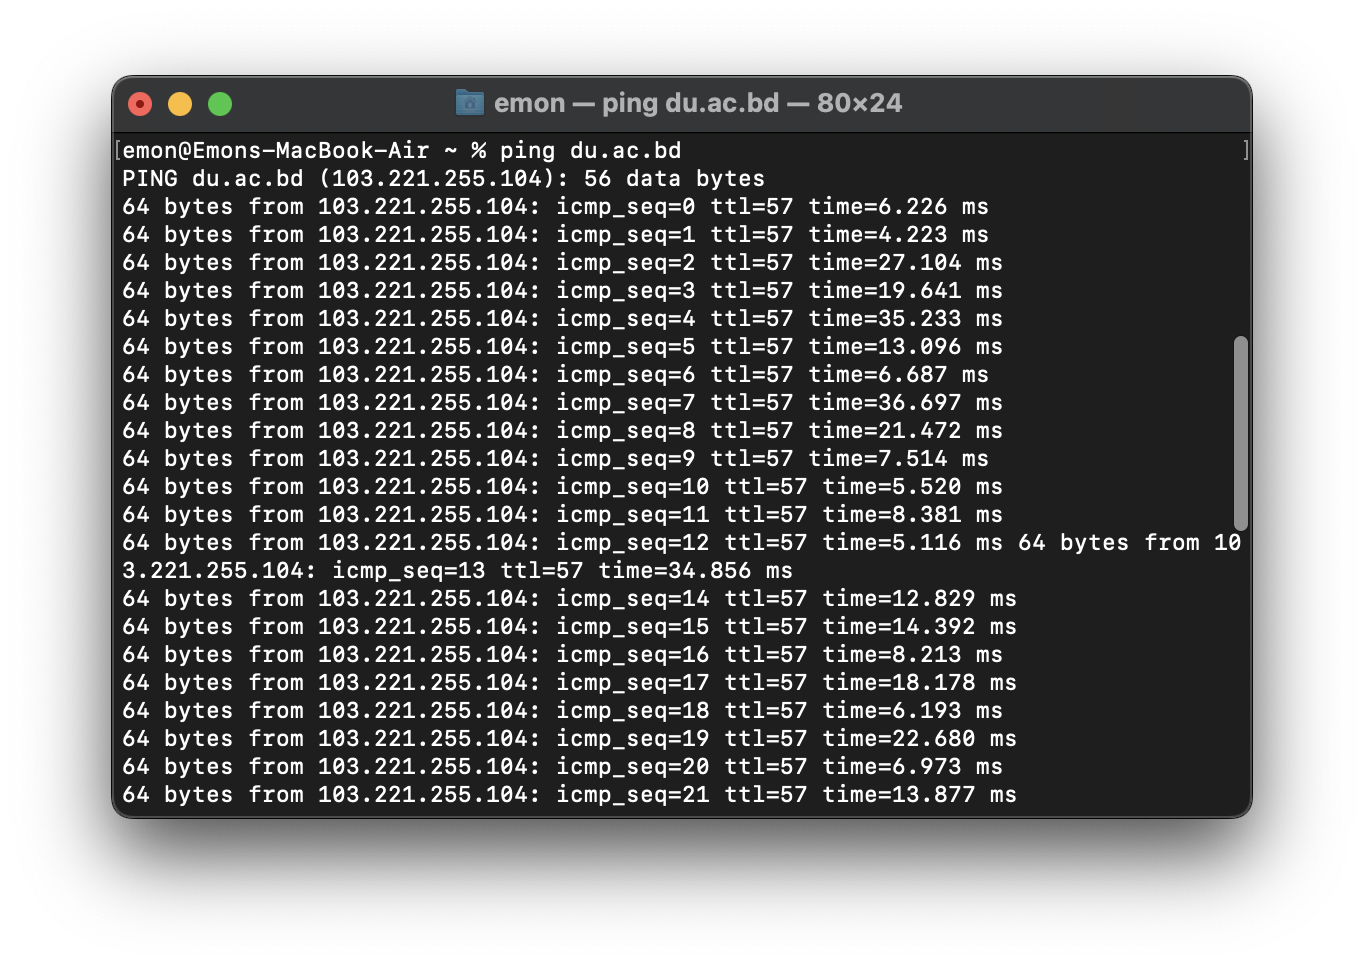
\includegraphics[width=\textwidth]{ping1.png}
    \caption{This sends a series of ICMP Echo Request messages to the specified domain and displays the round-trip time for each message.}
\end{figure}

\newpage
\subsubsection{Ping with Specific Count: \terminal{ping -c 5 google.com}}
\begin{figure}[!h]
    \centering
    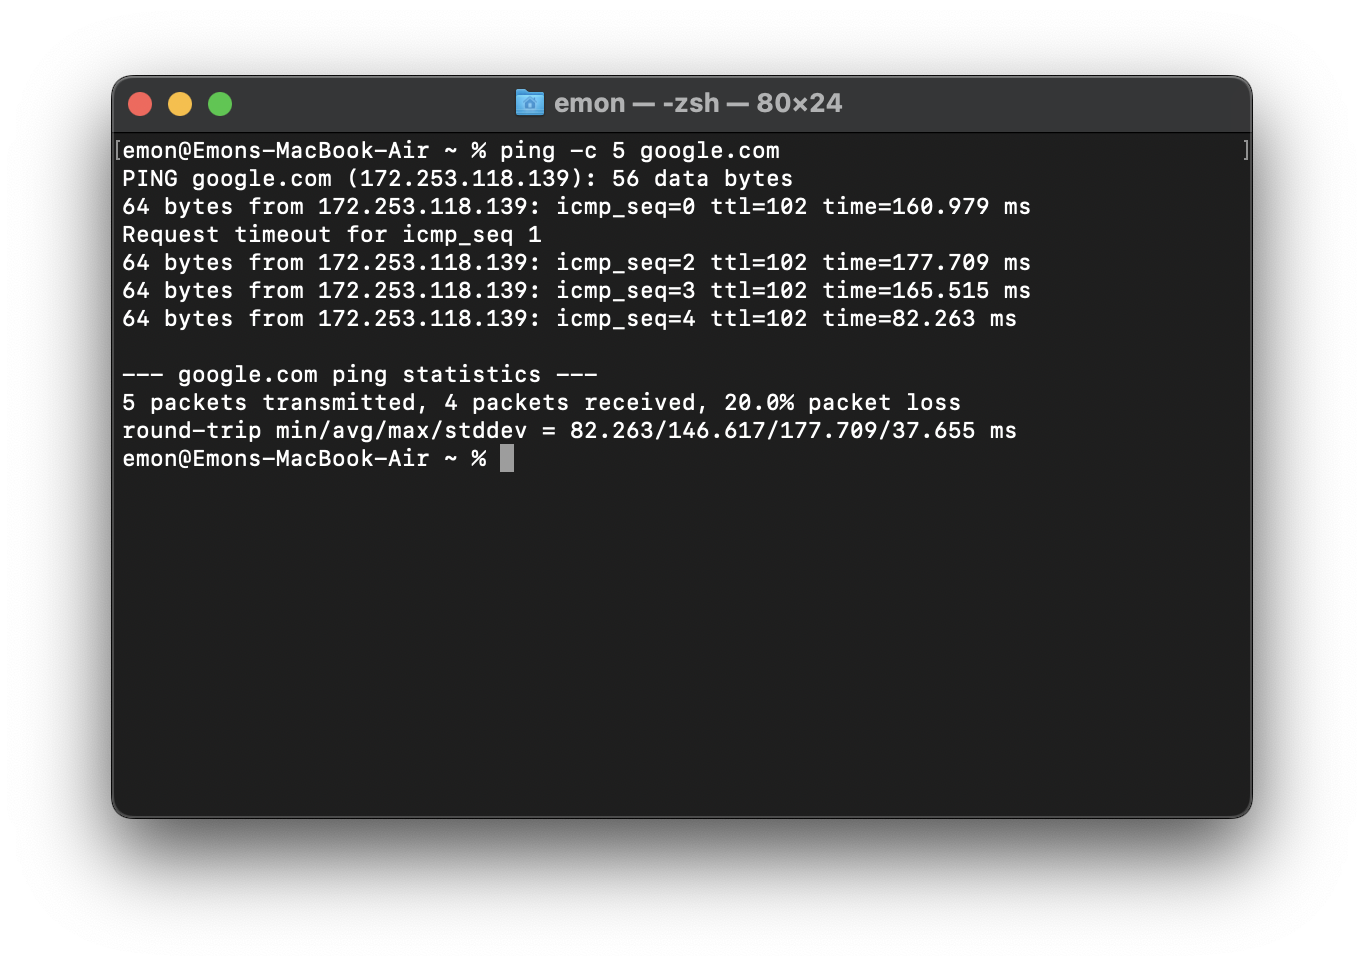
\includegraphics[width=\textwidth]{ping2.png}
    \caption{This sends only 5 ICMP Echo Request messages to google.com and then stops}
\end{figure}

\newpage
\subsubsection{Ping with Interval: \terminal{ping -i 2 facebook.com}}
\begin{figure}[!h]
    \centering
    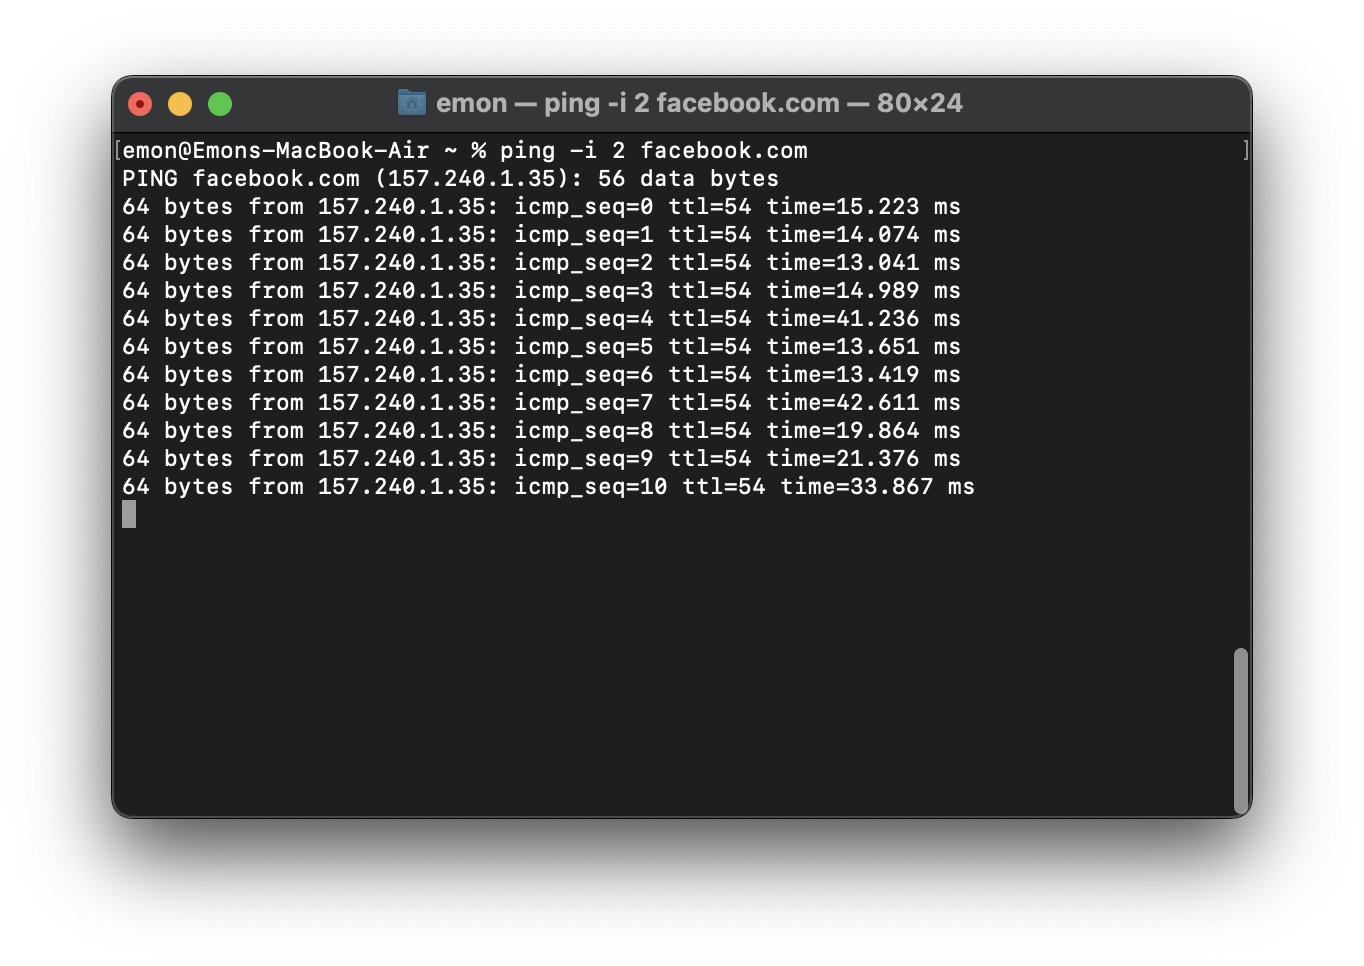
\includegraphics[width=\textwidth]{ping3.png}
    \caption{This sends ICMP Echo Request messages to facebook.com with a 2-second interval between each message.}
\end{figure}

\newpage


\subsection{Traceroute}
The \terminal{traceroute} is a network diagnostic tool used to track the route taken by packets in an IP network from the source to the destination. It provides information about the number of hops, round-trip times
\subsubsection{\terminal{traceroute google.com}}
\begin{figure}[!h]
    \centering
    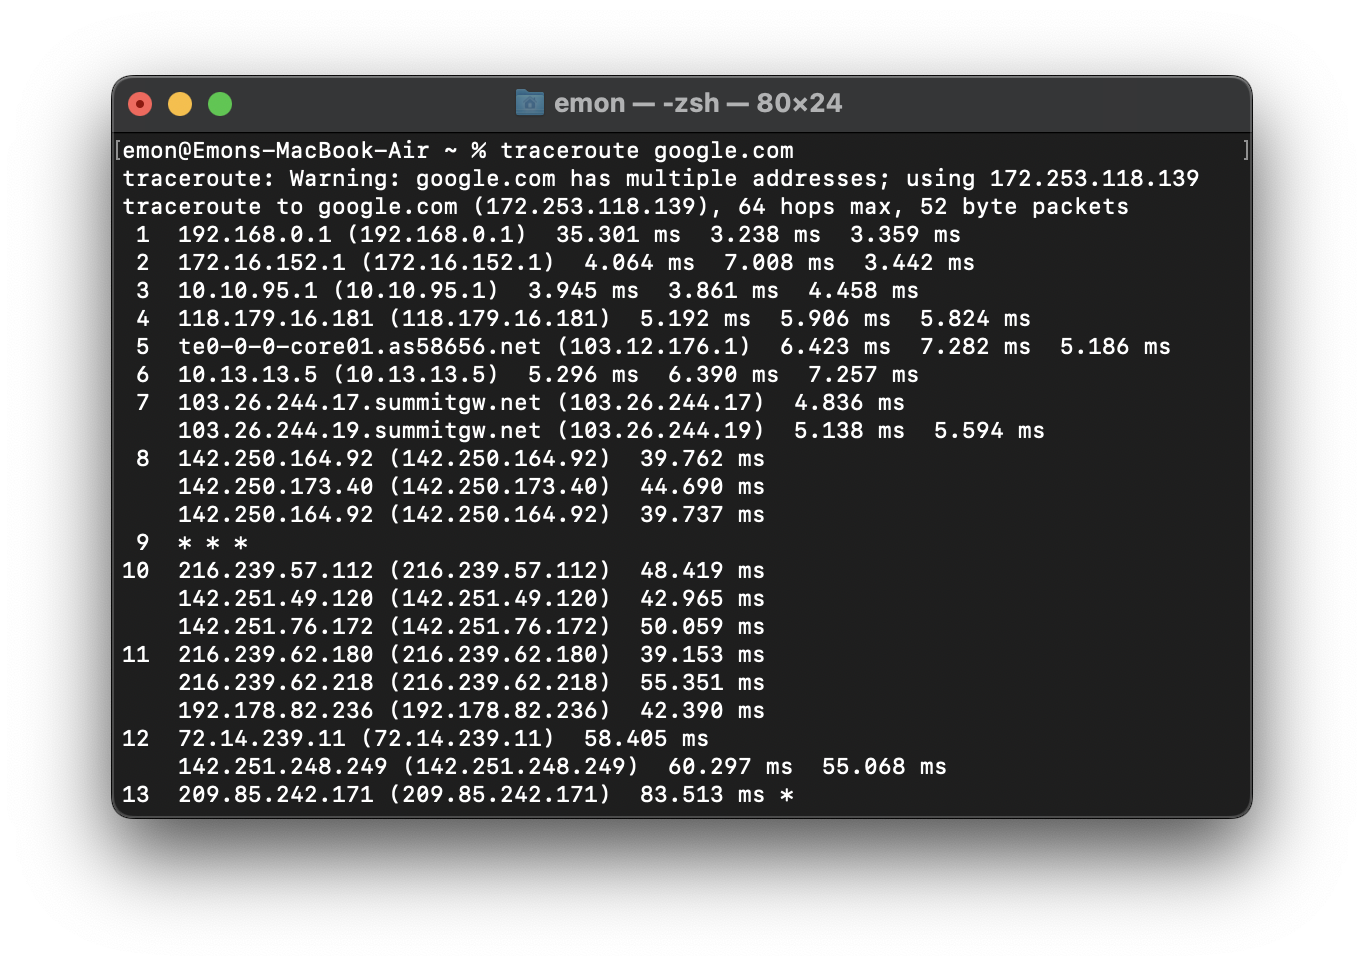
\includegraphics[width=\textwidth]{traceroute1.png}
    \caption{This command traces the route to the server of google.com, displaying the IP addresses and round-trip times for each hop.}
\end{figure}

\newpage

\subsection{IfConfig}
\terminal{ifconfig} (interface configuration) is a command-line tool that allows users to configure and display information about network interfaces on a system. It enables users to perform tasks such as configuring IP addresses, creating aliases, setting hardware (MAC) addresses, and enabling or disabling interfaces.
\subsubsection{\terminal{ifconfig}}
\begin{figure}[!h]
    \centering
    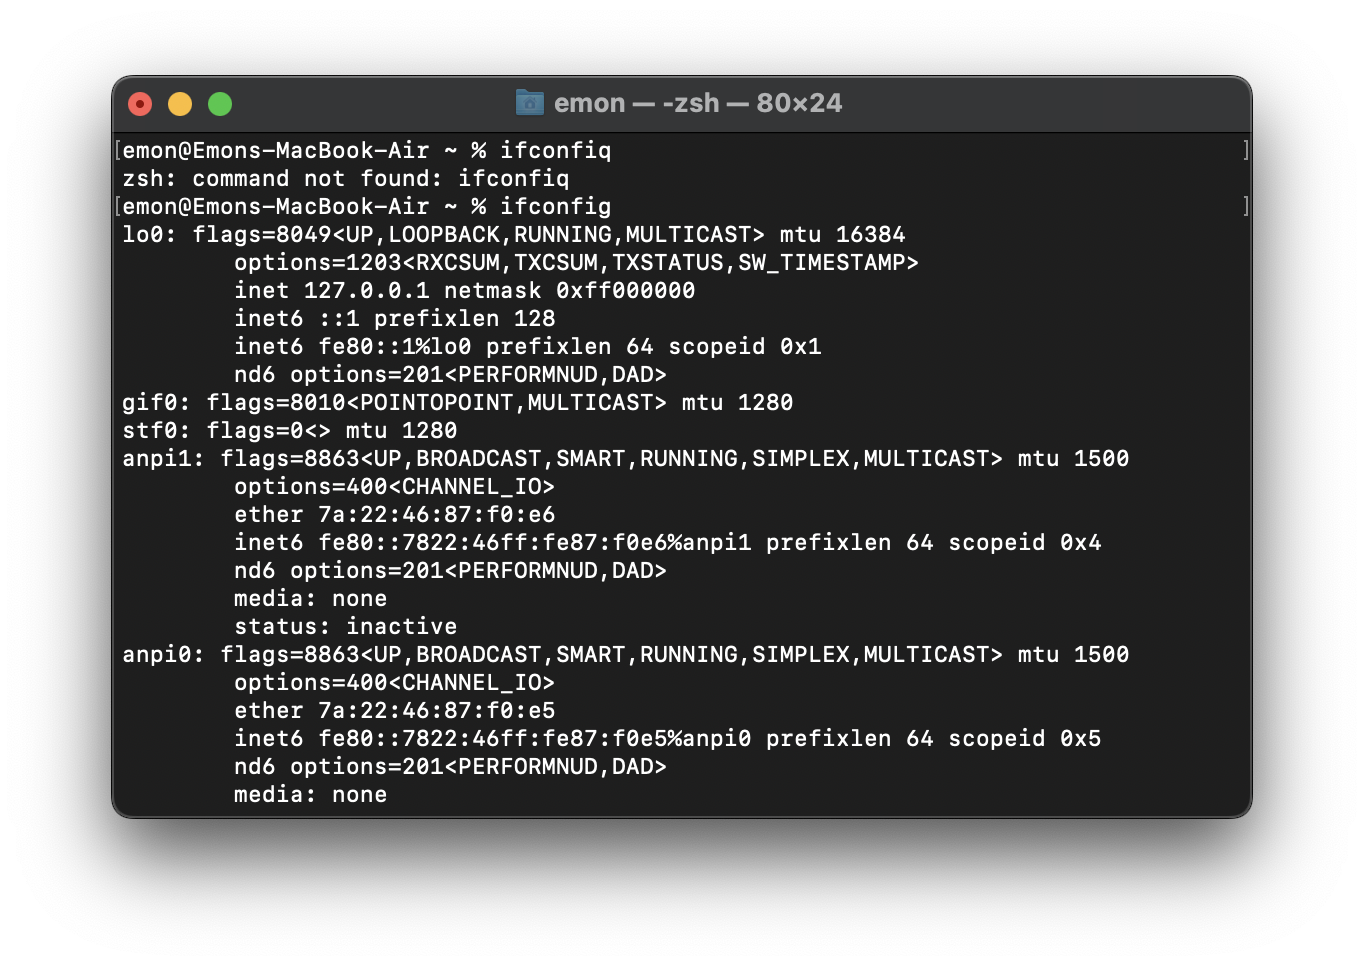
\includegraphics[width=\textwidth]{ifconfig1.png}
    \caption{The \terminal{ifconfig} command with no arguments will display all the active network interface configuration details. This includes loopback interfaces, software interfaces, network interfaces with hardware addresses (MAC), and Ethernet interfaces}
\end{figure}

\newpage

\subsubsection{\terminal{ifconfig -a}}
\begin{figure}[!h]
    \centering
    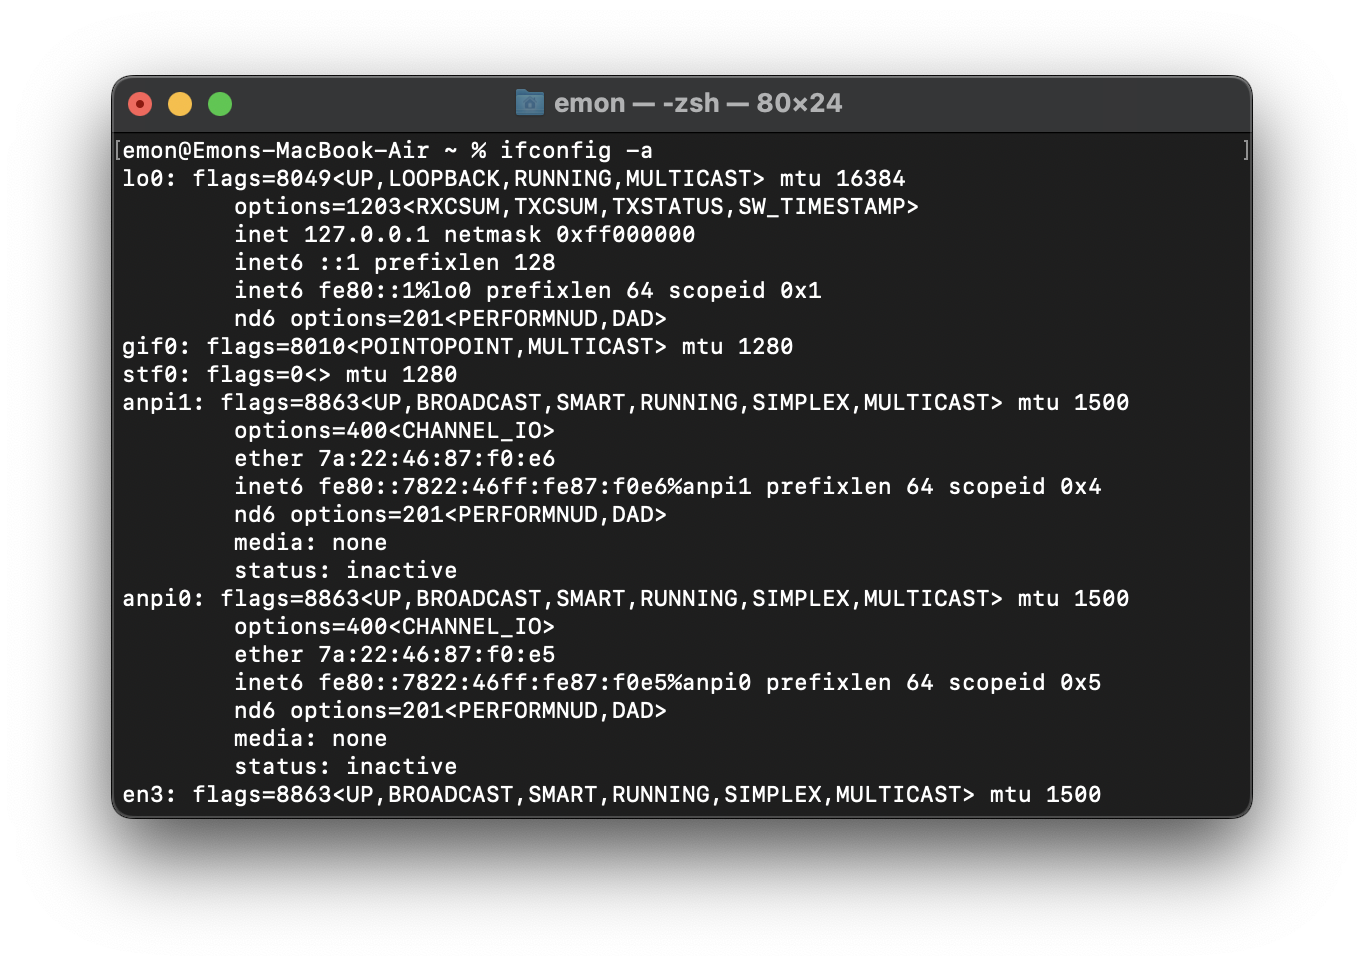
\includegraphics[width=\textwidth]{ifconfig2.png}
    \caption{The \terminal{ifconfig} command with the \terminal{-a} argument will display information on all active or inactive network interfaces on the server}
\end{figure}

\newpage

\subsection{arp}
\terminal{arp} command is used to display and manage the Address Resolution Protocol (ARP) cache. ARP is a protocol used to map an IP address to a physical (MAC) address on a local network.
\subsubsection{Display ARP Cache: \terminal{arp -a}}
\begin{figure}[!h]
    \centering
    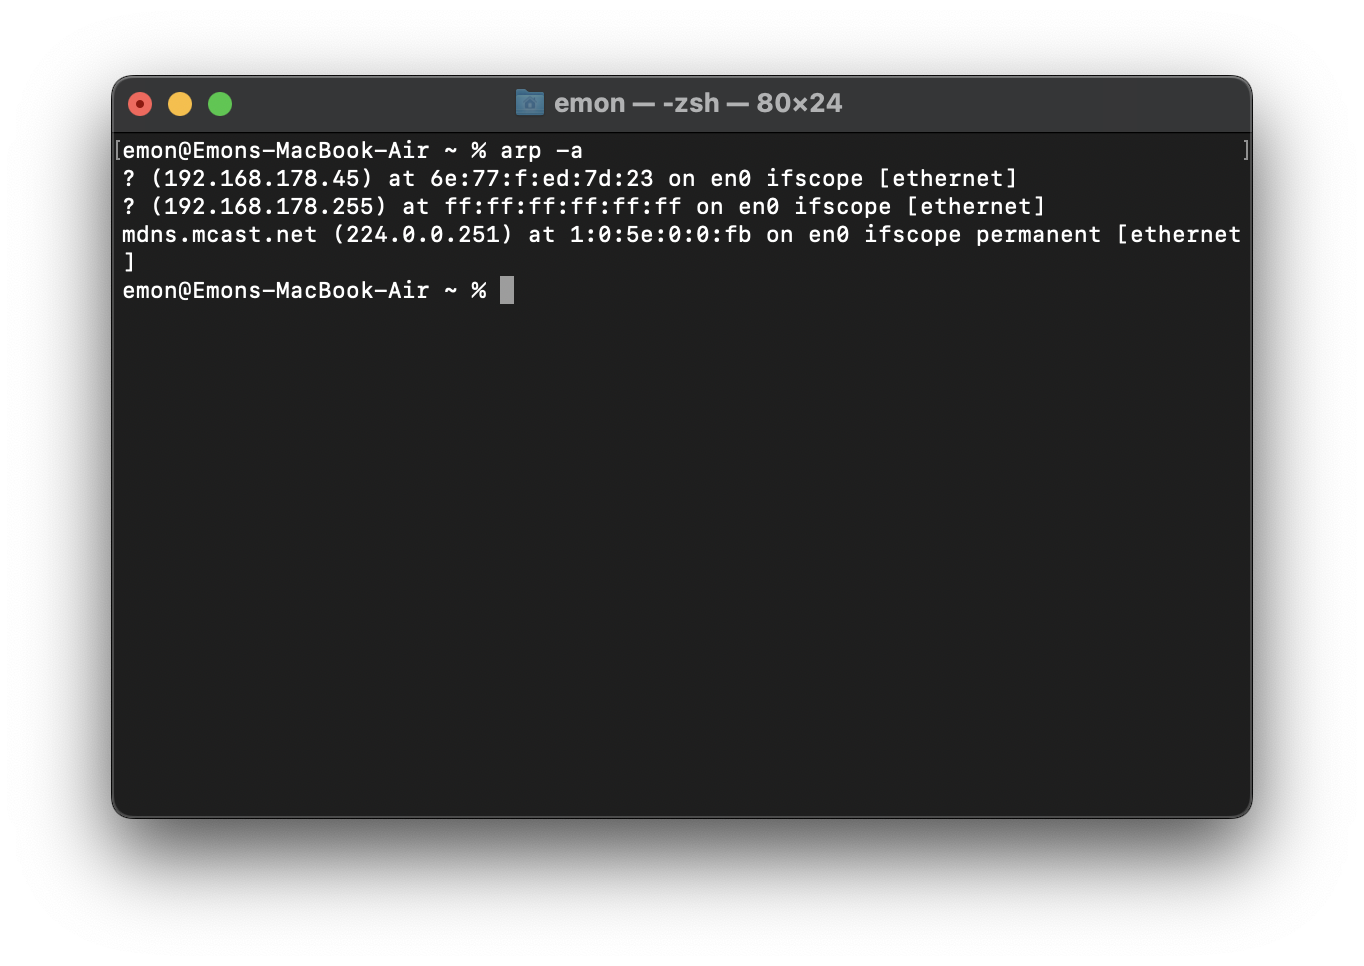
\includegraphics[width=\textwidth]{arp1.png}
    \caption{This will display a list of IP addresses and their corresponding MAC addresses.}
\end{figure}

\newpage

\subsubsection{Flush ARP Cache: \terminal{sudo arp -ad}}
\begin{figure}[!h]
    \centering
    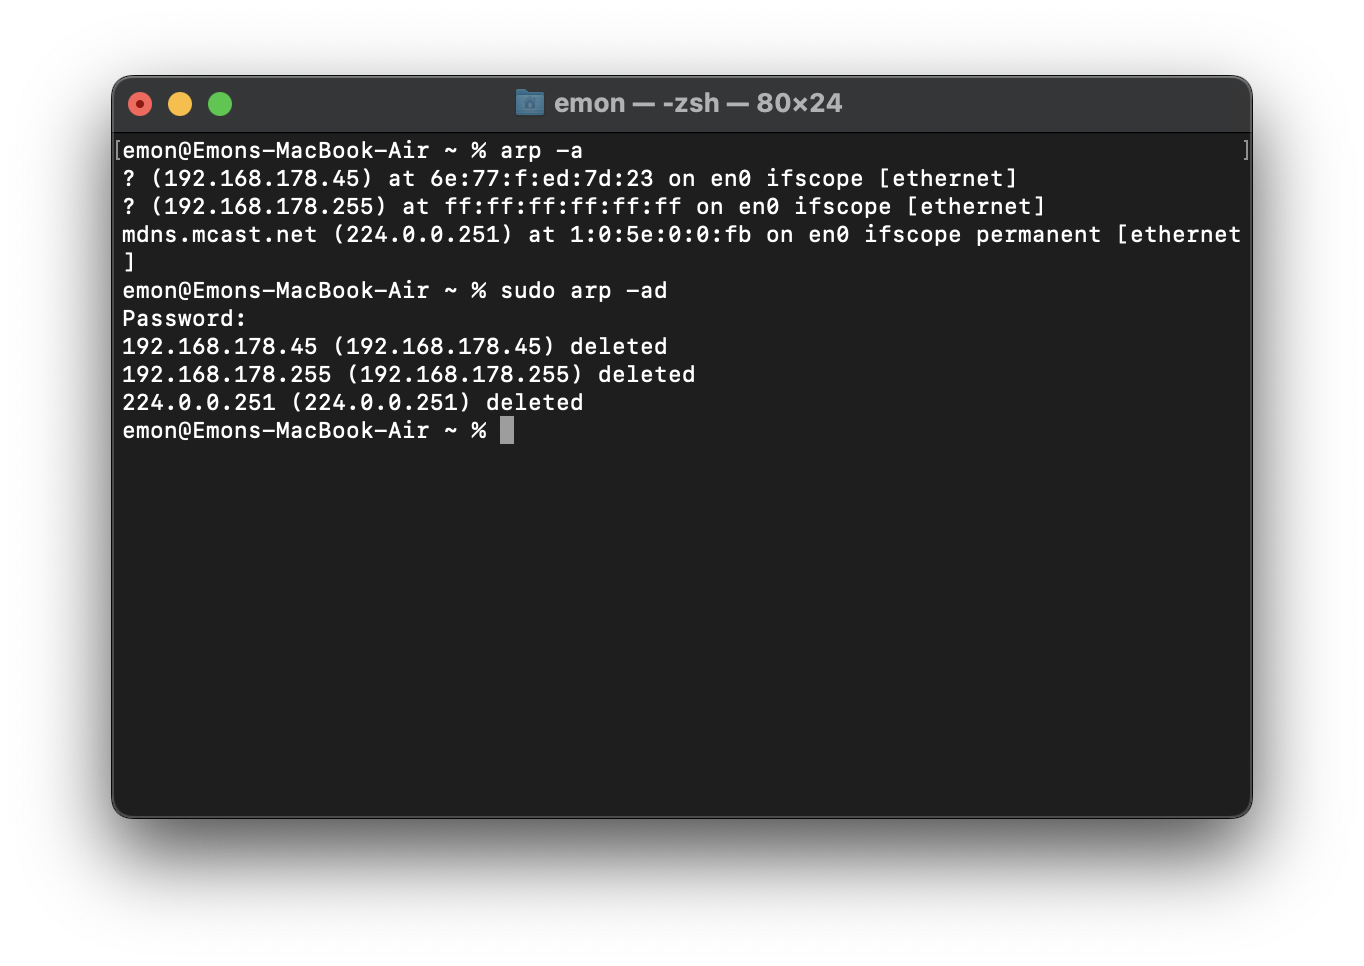
\includegraphics[width=\textwidth]{arp2.png}
    \caption{This command use to clear (flush) all entries in the ARP cache}
\end{figure}

\subsection{rarp}
\terminal{rarp}, or Reverse Address Resolution Protocol, is an obsolete networking protocol used in early computer networks. Its primary purpose was to map a device's physical hardware address (usually its MAC address) to its corresponding IP address.

\newpage


\subsection{Nslookup}
\terminal{nslookup} (stands for “Name Server Lookup”) is a useful command for getting information from the DNS server.It is used for querying DNS (Domain Name System) servers to obtain domain name or IP address mapping, DNS records, and other information related to domain names.
\subsubsection{\terminal{nslookup du.ac.bd}}
\begin{figure}[!h]
    \centering
    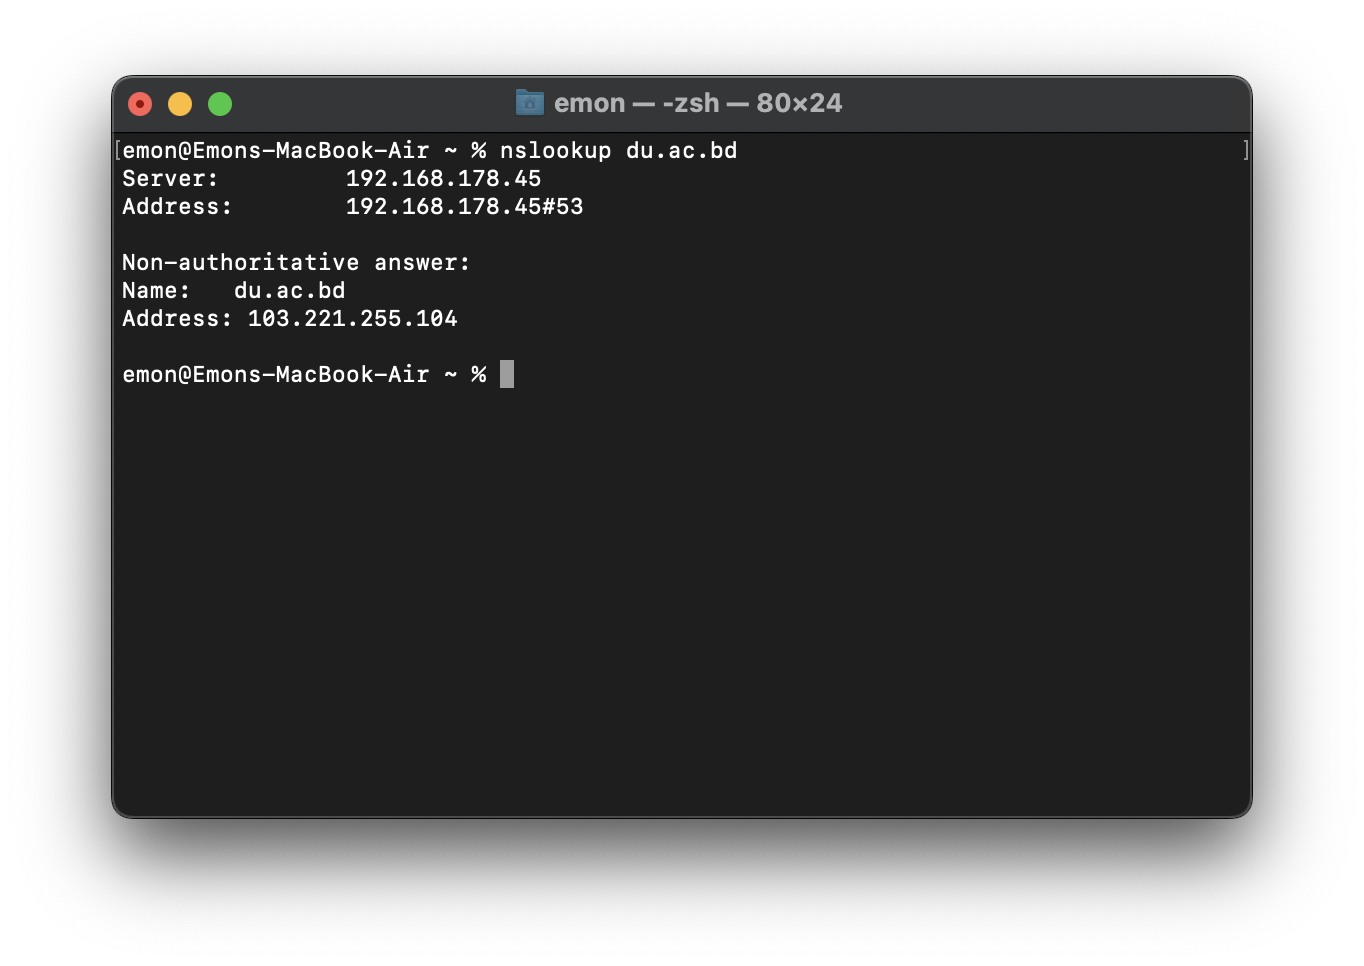
\includegraphics[width=\textwidth]{nslookup.png}
    \caption{The DNS server being used for the query is at the IP address 192.168.178.45, and it operates on port 53, the standard port for DNS. The domain "du.ac.bd" resolves to the IP address 103.221.255.104. This is the information obtained from the DNS server.}
\end{figure}

\newpage



\subsection{Netstat}
The \terminal {netstat}  command is a network utility tool used to display information about network connections, routing tables, interface statistics, masquerade connections, and multicast memberships.
\subsubsection{\terminal{netstat -an}}
\begin{figure}[!h]
    \centering
    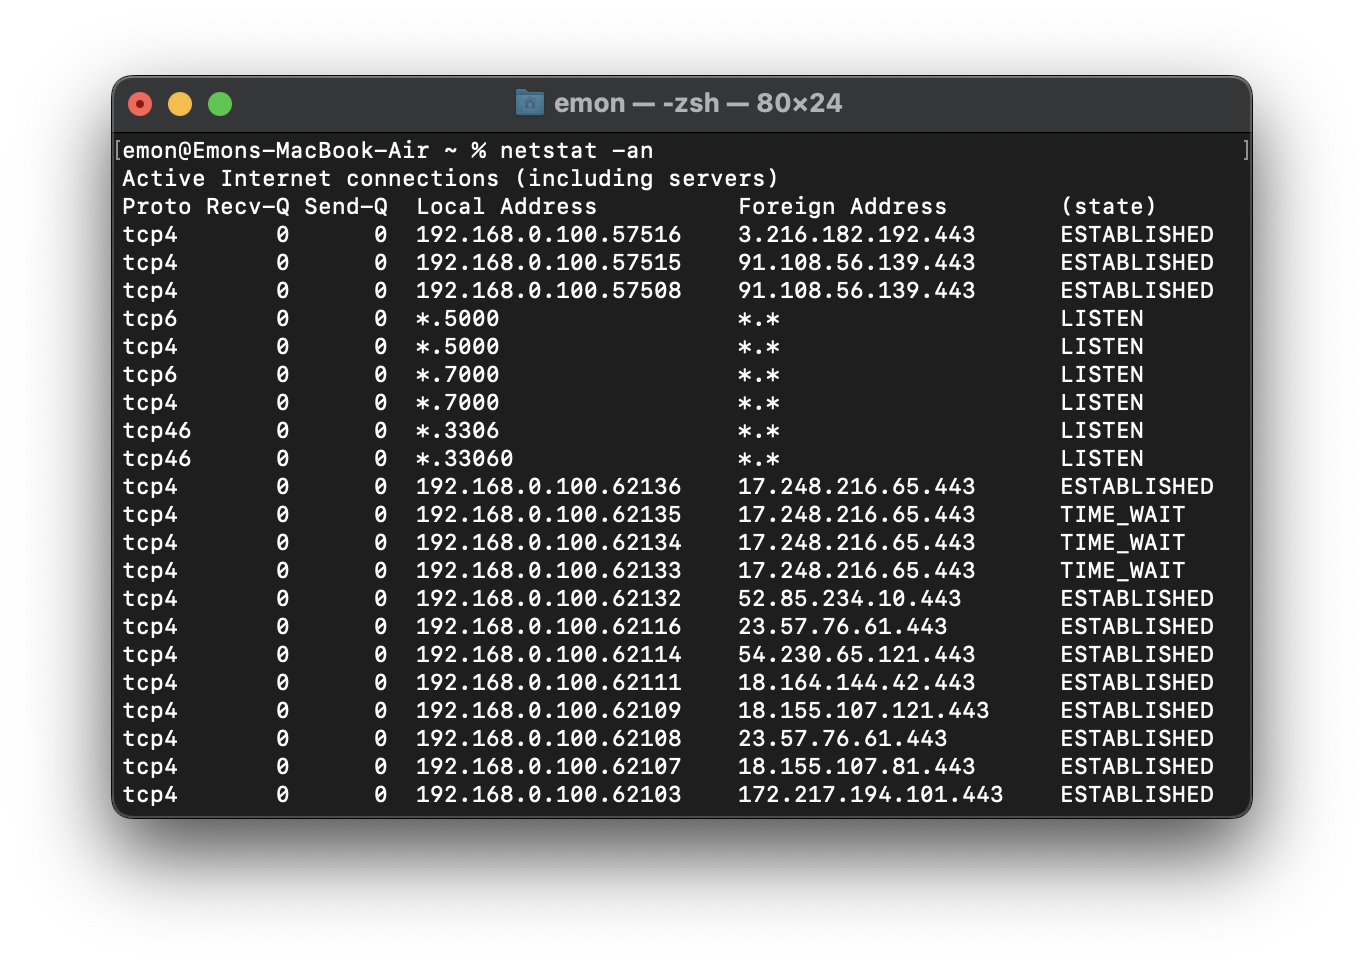
\includegraphics[width=\textwidth]{netstat1.png}
    \caption{This command displays a list of all active network connections, along with their local and remote IP addresses and port numbers}
\end{figure}

\newpage

\subsubsection{\terminal{netstat -s}}
\begin{figure}[!h]
    \centering
    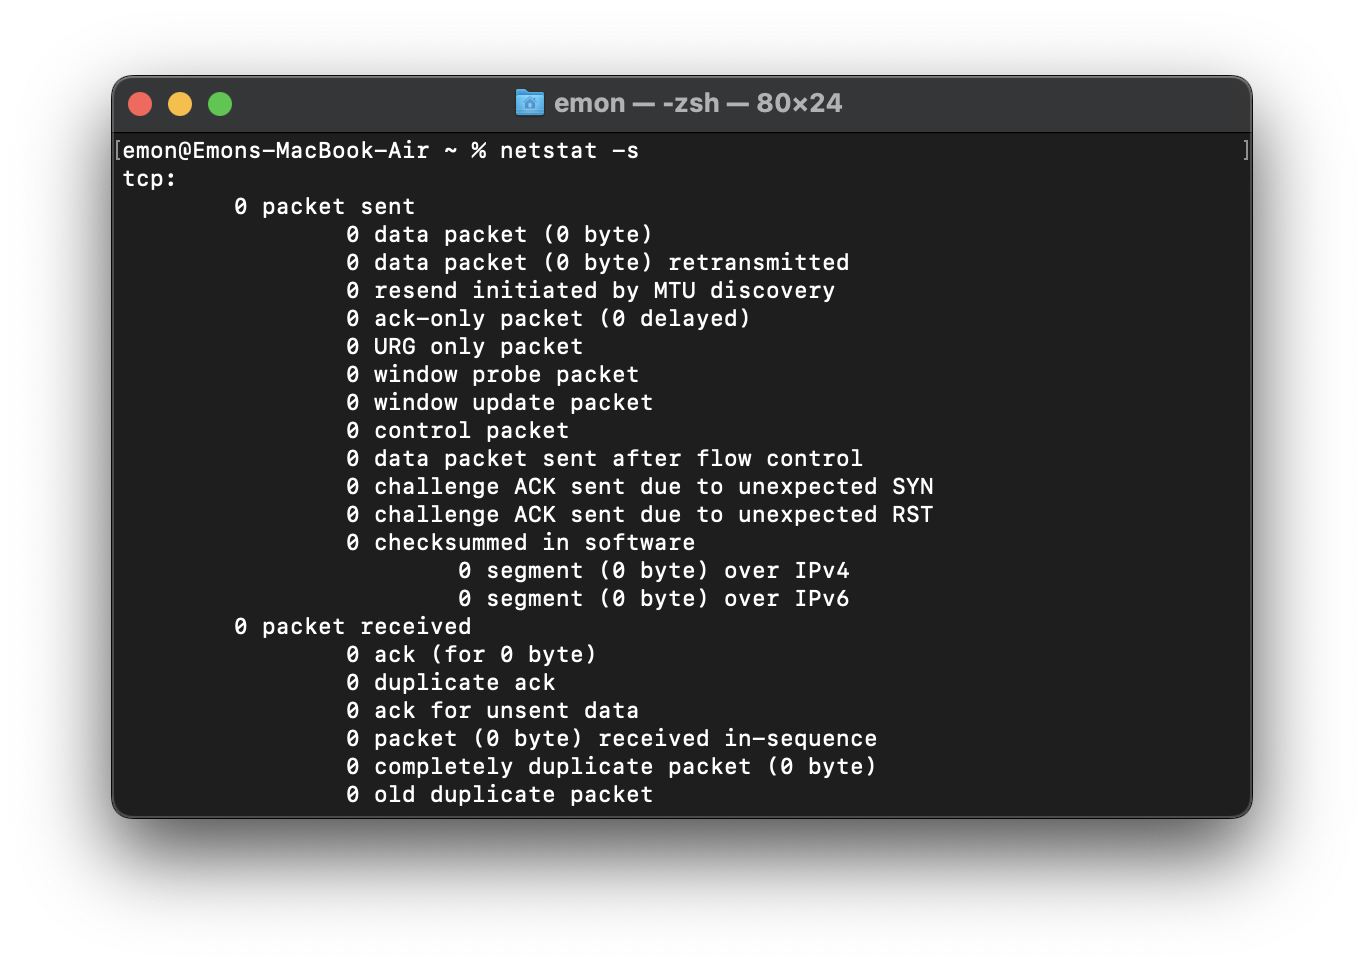
\includegraphics[width=\textwidth]{netstat2.png}
    \caption{This command displays statistics for each protocol, including the number of packets sent and received.}
\end{figure}

\newpage

\section{Experience}
\begin{enumerate}
    \item We had to see some examples of how to use the tools in the command line
    \item We used these commands for the first time to actually find the LAN configurations
\end{enumerate}

\begin{thebibliography}{1}
    \bibitem{Pi My Life Up}  \url{https://pimylifeup.com/}
    \bibitem{Cloud Infrastructure Services} \url{https://cloudinfrastructureservices.co.uk/}
    \bibitem{Tecmint} \url{https://www.tecmint.com/}
    \bibitem{Geeks For Geeks} \url{https://www.geeksforgeeks.org/}
\end{thebibliography}

\end{document}
